\section{Gitter}

Fælles for alle 3 systemer er kølegitteret af aluminium, der er i kontakt med processoren. 
I simple systemer udgør kølegitteret den eneste part i kølesystemet som vi har defineret det og kan selvfølgelig bestå af andre materialer end aluminium. I nærværende rapport vil der dog tages udgangspunkt i aluminum.

Kølegitteret udnytter sit store overfladeareal til at bortlede varme ved konvektion fra et fast materiale (aluminium) til et fluid (tør atmosfærisk luft).
Således vil der være to termiske modstande, nemlig en varmeledningsmodstand i kølegitteret og en varmeovergangsmodstand fra fast stof til fluid.

En hyppig forekommende geometrisk struktur i et kølegitter er ribber eller lameller, der giver en naturlig strømning af den varme luft bort fra kølegitteret, hvor kun termodynamiske kræfter har indflyldelse på strømningen. Denne strømning foregår mellem to ribbe/lamel-vægge. 

Der præsenteres her en oversigt over de værdier der bruges i udregningerne: 

Der beregnes varmestrøm for konvektion og for stråling.

Dimensionerne for kølegitteret er importeret fra en partfil i Solidworks. %Kanalen for strømningen af luft der regnes for er d(1mm) bred og den hydraulisk diameter regnes som værende en snæver kanal, hvor L=2*a

$H = 20\ mm$, $b = 25,5\ mm$, $d = 1\ mm$, Areal $A_t = 93733.73\ mm^2$, $A_{lamel}= 500\ mm^2$  \\ 
Massen $m = 31,58 g$ \\
Varmekonduktiviten for aluminium, $\lambda_{al} = 229\ W/m*K$ \\  
Lameltykkelsen $\delta = 0.5\ mm.$  \\
Den specifikke varmekapacitet $c_{p} = 1.008\ kJ/kg*K$ \\
Strømningshastighed lodret, i lamellens længde på $c = 0.001\ m/s$ \\

Varmekonduktiviteten $\alpha$ er fundet ved tabel opslag $\alpha = 21.8$ \\
Kinematisk viskositet er: $18.88$ og dynamisk viskositet = $16.92$  \\
Volumenudvidelseskoefficienten $\beta_luft = 3,2$ \\
 
Varmeledningsmodstanden : $R_l = \frac{\delta}{\lambda_{al}*A_{lamel}} = 4.281$ \\
Varmeovergangsmodstanden : $R_o = \frac{1}{\alpha_{tl}*A_{lamel}} = 89.394$ \\

Total termisk modstand er $R_{tot} = R_l + R_o = 92.225$ \\

\section{Beregninger}

For at udregne varmestrømmen $\phi$  bruges udtrykket \\ $\Phi = \alpha * A* (t\_{fl}-t\_v$ \\  også kendt som Newtons ligning. \\ 

Varmestrømmen $\phi$ udregnes ved ligningen Nu = $\frac{\alpha}*{\lambda}$ \\
Nu er Nusselts tal og findes herunder ved at udregne Reynolds(Re) og Prandtls(pr) tal.

Strømningsforholdende for luft(fluiden) imellem lamellerne i gitteret er fri indvendig strømning, idet lamellerne kan ses som kanalvægge og udgangen i en antaget lodret given retning er smal og bred med 3 åbne sider og derved tillader en fri udvikling af strømningen. Den hydrauliske diameter bruges og sættes lig med afstanden imellem 2 givne lameller. $\approx 0.5 mm$

Reference temperaturen udregnes til : 
\\$t_{film} = \frac{{t_{lamel}}+t_{fluid}}{2} => t_{film}=30$
\\Grasshofs tal Gr = $\frac{g*L^3*\beta*{\Delta\,t}}{\upsilon\,^2} = 8,771*10^4$
\\Prandtls tal Pl(opslag) => $Pr=0.69$

Der antages lodret laminar strømning af luften og Reynold tal undersøges for at få en idé om strømningsformen\\

$Re = \frac{c_{luft}*L_{hyd}}{\upsilon} = 2.648*10^{-5}$
%$ Ra = Gr*Pr = 6.052*10^4$ => \\ 

Den kritiske værdi for Re hvor strømningen overgår fra at være laminar til at blive turbulent er $10^9$.  Da ovenstående beregnede værdi af Re er meget mindre end den kritiske værdi, ses at der må være tale om laminar strømning over hele længden af en lamel, hvorfor strømningen ikke undersøges yderligere.

Hastighedsprofilen hvorved den opvarmede luft stiger til vejrs er udregnet til: 
$0.05*Re*L_{hd} = 0.001 $

Her følger et overblik over forksellene på to strømningsformer.

\subsection{Tvungen indvendig strømning}
Det medfører at Nusselts tal kan udregnes som \\ 
$Nu = 3,66+ \frac{0.0668*Re*Pr*\frac{D}{L_{lamel}}}{1+0.004*()\frac{D}{L_{lamel}}*k *Re*Pr})^{2/3} = 3.661$


%Den kritisk værdi findes da ved: $Nu_m = C*Ra^4$

og $ \Phi_{tis} = \alpha*A(t_{fl}-t_v =>2.597*10^6 W $\\ 
justeret til milimeter ved udtrykket: $\frac{\Phi = \alpha*A*(t_{fl}-t_v}{10^6} =>160,4 W$

Hvor luftens hastigheds profil er fuldt udviklet efter :
$0,05*Re = 0,03 mm$

samtlige lameller afgiver da $0,75 w* 40 \approx 30 W$ i varmestrøm til luften der passerer. 

\subsection{Fri Konvektion}

Fri konvektion er et lidt tænkt scenarie, som er lidt begrænset i sin relevans men dog brugbar for enkelt-lameller og dele af kølegitteret.

$Nu_{fri} = (\frac{Gr_{L}}{4})^4 * (\frac{0,75*Pr^1/2}{(0.609+1,221*Pr^1/2+1,238*Pr)})^1/4$
og ledetallet $\alpha_{fri} = 2,768*10^3$

Varmestrømmen $\phi_{fri}=169,37$

\begin{figure}
	\centering
	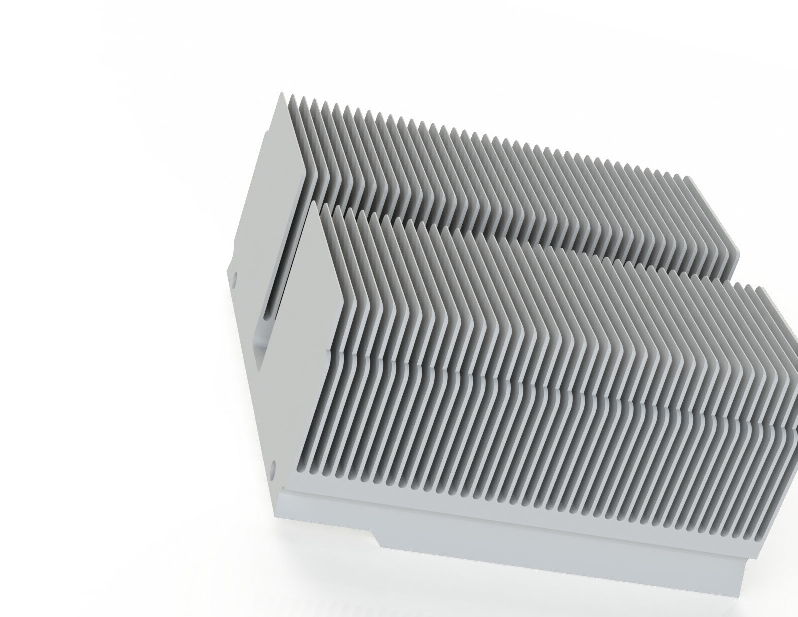
\includegraphics[width=0.7\linewidth]{billeder/heatsink1}
	\caption{Eksempel på kølegitter, Fra grabcad.com - bruger: Fernando}
	\label{fig:heatsink1}
\end{figure}

\begin{figure}
	\centering
	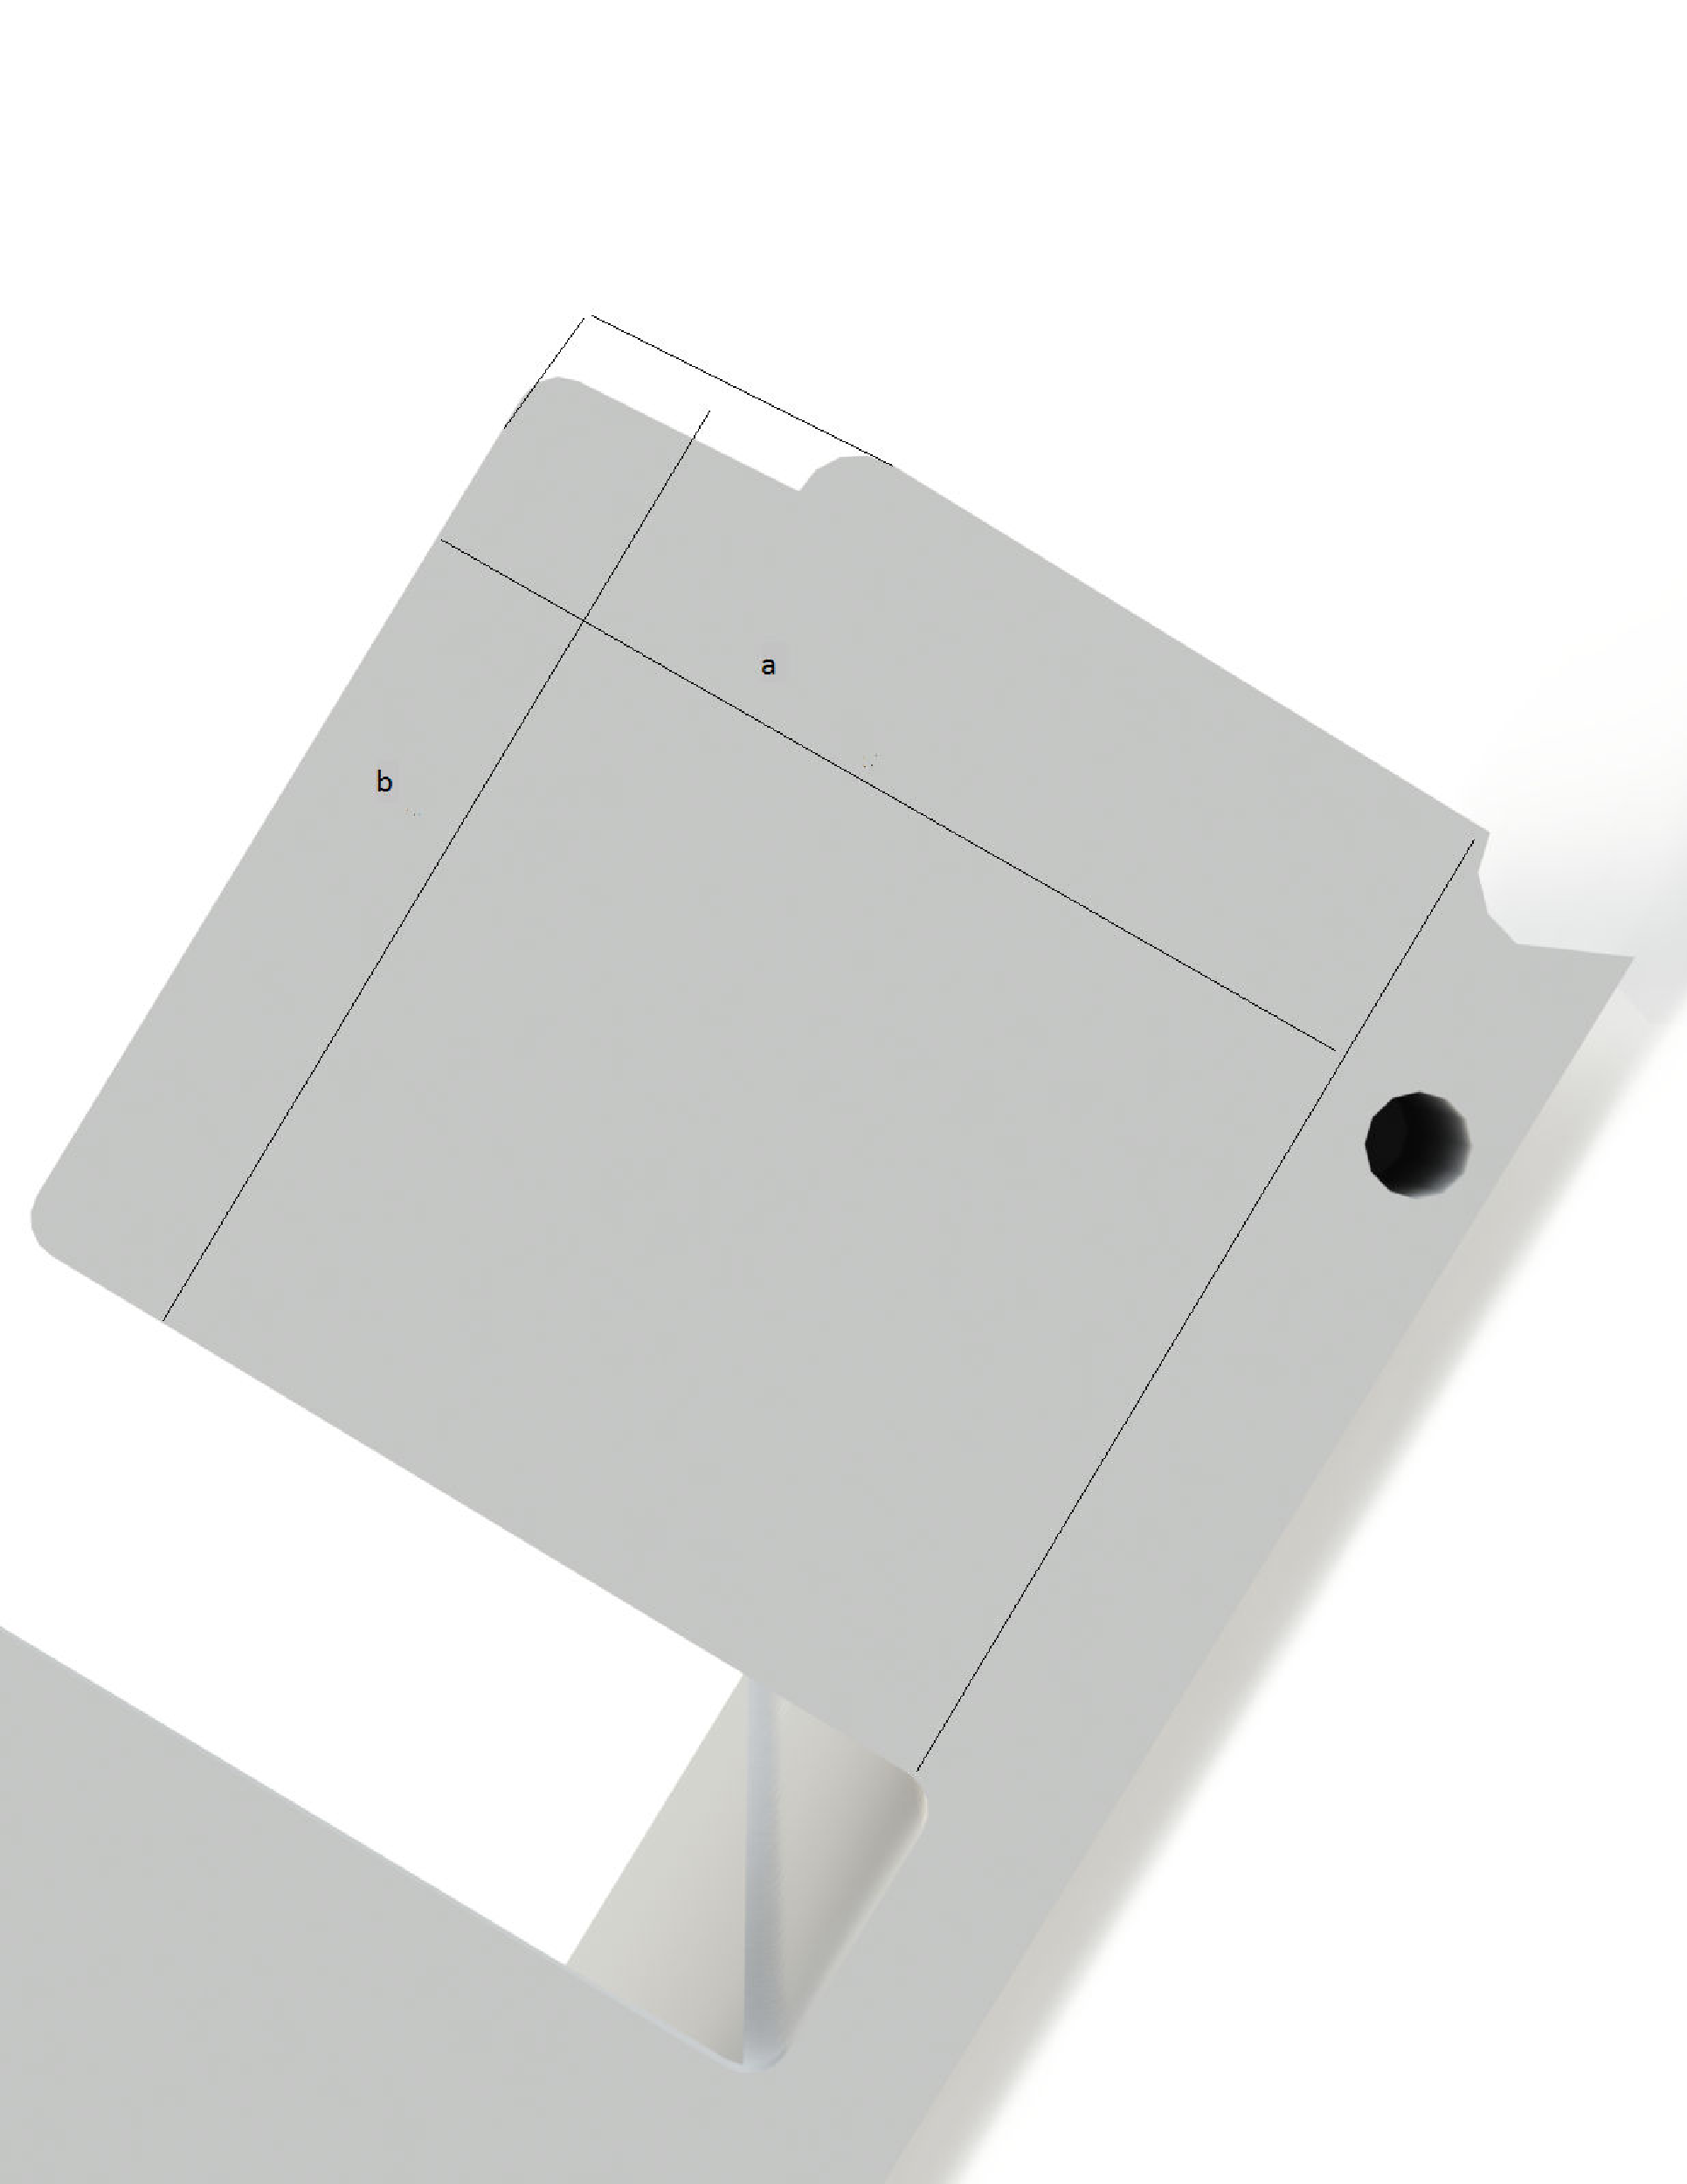
\includegraphics[width=0.7\linewidth]{billeder/lamel}
	\caption{Lamel. Genstand for vore termdynamiske undersøgelser. Fra grabcad.com - bruger: Fernando}
	\label{fig:lamel}
\end{figure}
